% Commands:
%
% * EtherstubManager._create( name );
% * VnicManager._create( name, temporary, parent );
%
% * one worker instantiation: switch + 2 appliances + communication     (sim)
% * two workers instantiation: (dou)


\documentclass{beamer}

\usepackage[polish]{babel}
\usepackage[utf8]{inputenc}
\usepackage[T1]{fontenc}
\usepackage{hyperref}
\usepackage{graphicx}
\usepackage{multicol}
\usepackage{tabularx}
\usepackage{tikz}

\usetikzlibrary{positioning}

\mode<presentation>{\usetheme{Dresden}}
\setbeamercovered{dynamic}

\title{Component-based system for management of multilevel virtualization of networking resources}
\subtitle{System komponentowy wspomagający wielopoziomową wirtualizację zasobów sieciowych}
\author{Robert Boczek \and Dawid Ciepliński \\ ~ \\ prof. dr hab. inż Krzysztof Zieliński}
\date{10.05.2011}

\begin{document}

	\begin{frame}
		\titlepage
	\end{frame}


	\begin{frame}{The environment}

		\begin{enumerate}

			\item ,,Physical''

				5 Logical Domains connected with a vswitch:

				\begin{itemize}
					\item dedicated NFS server node (virtual appliance snapshot storage)
					\item 4 worker nodes
				\end{itemize}

				\begin{center}
				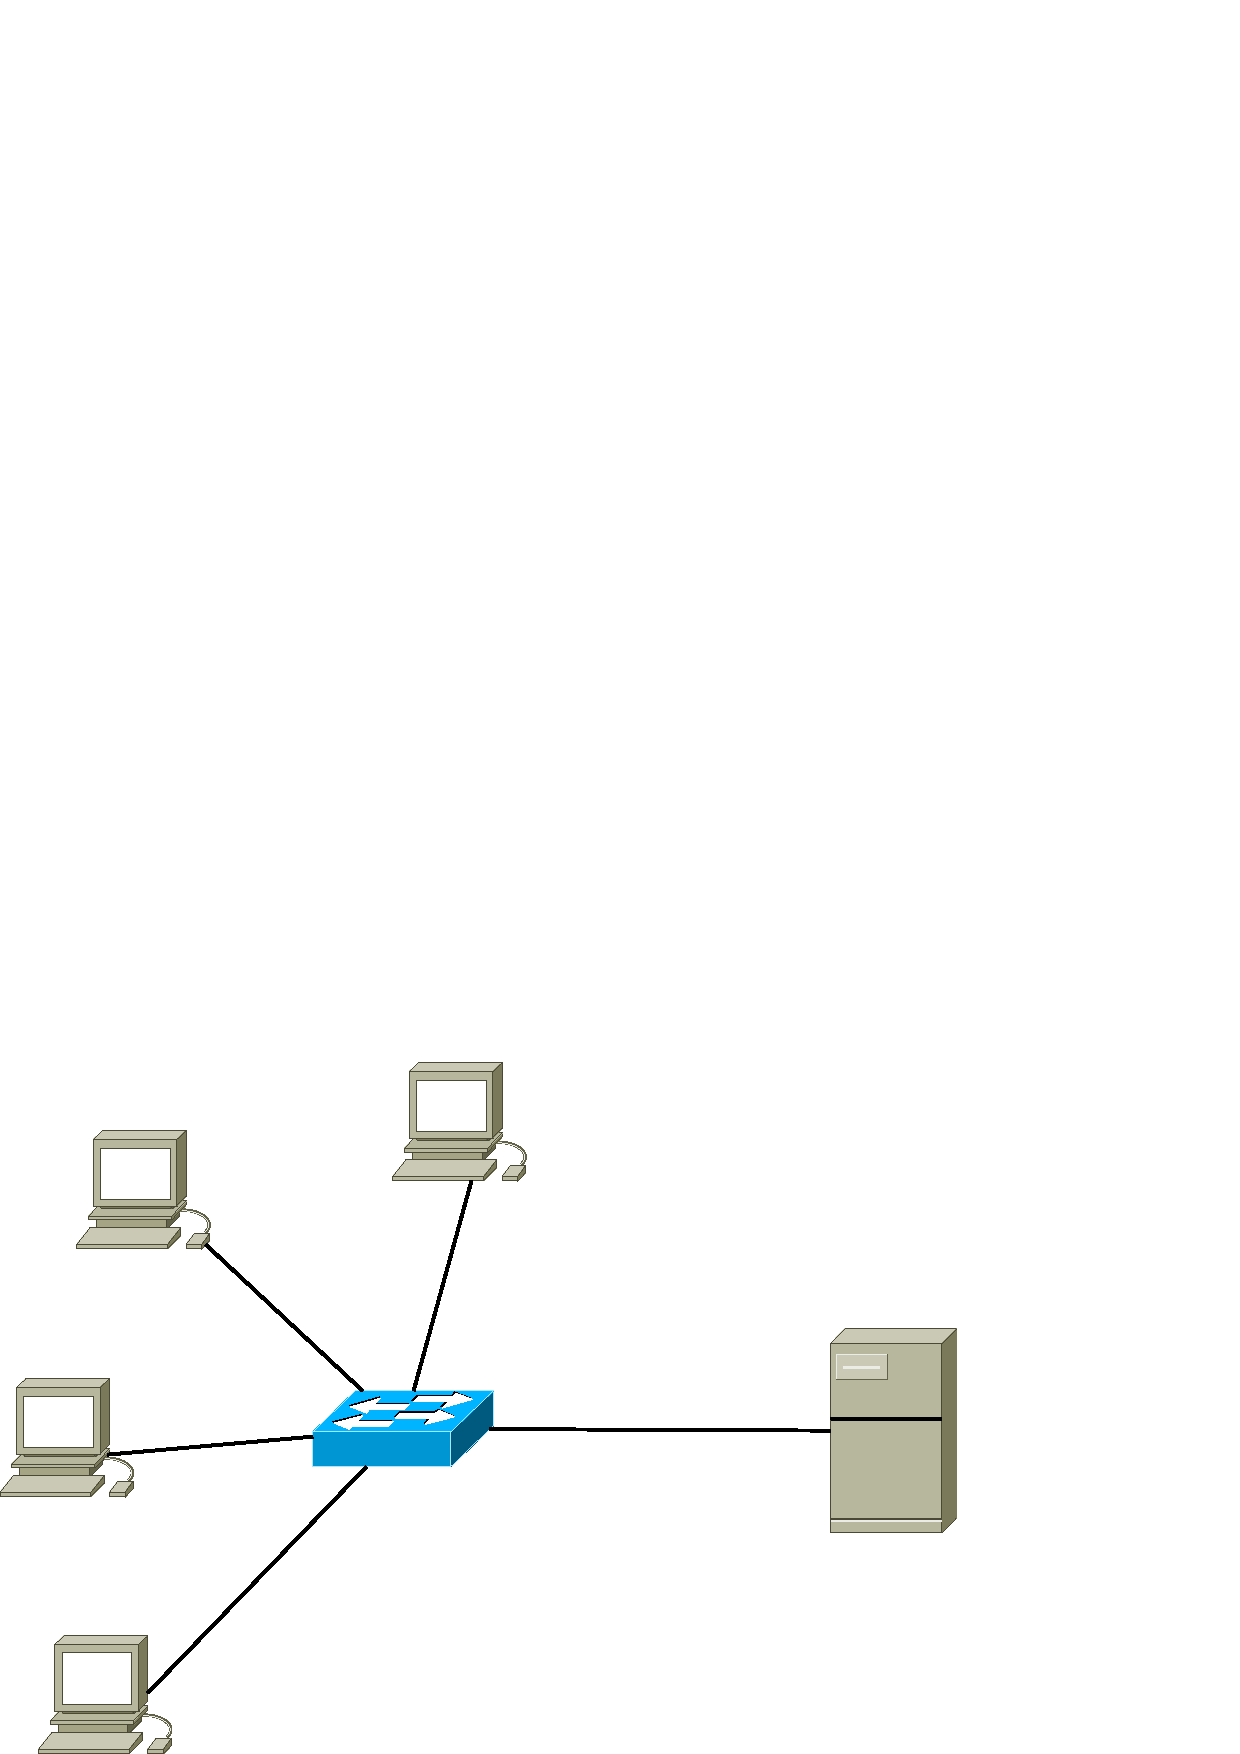
\includegraphics[scale=.2]{img/env.pdf}
				\end{center}

				\pause

			\item Software = JMX-enabled Monitoring System (JIMS)

				\begin{itemize}
					\item Solaris resource monitoring \& management (containers)
					\item peer discovery
					\item shared codebase
				\end{itemize}
		
		\end{enumerate}

	\end{frame}


	\begin{frame}{Native libraries}

		\texttt{libdladm}- and \texttt{libflowadm}-based native libraries.

		\begin{itemize}
			\item lib-link
			\item lib-etherstub
			\item lib-flow
			\item lib-vlan
		\end{itemize}

		Allow for higher-level operations (CRUD) for etherstubs, (V)NICs, VLANs and flows. Still native, with minimum external dependencies.
	
	\end{frame}


	\begin{frame}{MBeans}

		Two kinds:
		
		\begin{enumerate}
			\item managers: entity discovery \& general management
			\item entities: fine-grained control (properties, statistics)
		\end{enumerate}

		Bidirectional operations.
	
	\end{frame}


	\begin{frame}{Components (simplified)}

		go here
	
	\end{frame}


	\begin{frame}{Remaining work}

		\begin{enumerate}
			\item statistics, charts (ongoing)
			\item parallelization
			\item usability improvements
			\item bug fixing
		\end{enumerate}
	
	\end{frame}


\end{document}

